\sloppy
French astronomer Charles Messier's
Catalogue des N{\'e}buleuses et des Amas d'{\'E}toiles (Catalog of Nebulae and
Star Clusters) contains 104 objects visible over the Parisian night sky that
were frequently encountered during his efforts as a comet hunter.
Although compiled in the
eighteenth century and officially published from his personal notes in
\citeyear{Messier},
the positions and characterizations of objects given by \citet{Messier} are
well-enough described that they are all easily and frequently
observed today by amateur astronomers across the planet. One such object carries the following
description (translated from the original French and sourced from
\texttt{http://www.messier.seds.org/xtra/history/m-cat81.html}):
\begin{displayquote}
    It is double, each has a bright center, which are separated
    $4^{\prime}35^{\prime\prime}$.
    The two \say{atmospheres} touch each other, the one is even fainter than the
    other \cite{Messier}.
\end{displayquote}
Of course, in the late eighteenth century, Messier would not be predisposed to
assuming that the \say{very faint nebula} with two touching atmospheres
he describes would be the often-imaged
interacting galaxy pair, Messier 51a and b.
Four years after \citet{Messier}, German philosopher Immanuel Kant only
theorizes that perhaps, the exceedingly dim yet huge \say{stars} are not
stars but seem to be most easily characterized as other Milky Ways \cite{kant}.
The main member of the pair is more colloquially referred to as the Whirlpool Galaxy, which is shown in figure \ref{fig: m51}.

\begin{figure}[h]
    \centering
    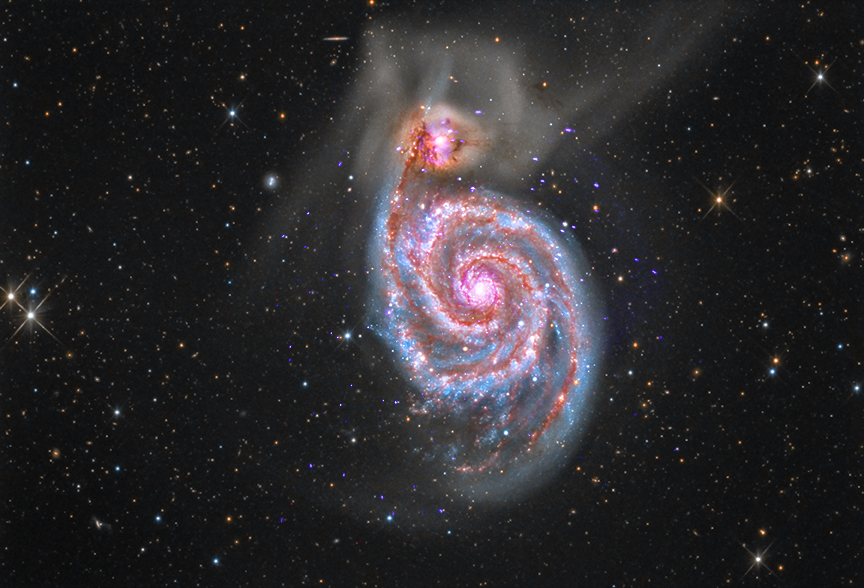
\includegraphics[width=0.5\textwidth]{m51.jpg}
    \caption[Composite image of Messier 51]
    {Composite image of Messier 51, The Whirlpool Galaxy. (Credit:
    X-ray: NASA/CXC/SAO; Optical: Detlef Hartmann; Infrared: NASA/JPL-Caltech)}
    \label{fig: whirlpool}
\end{figure}%


Galaxies are much less frequently found in isolation than they are found
in \textit{systems} of galaxies. We can therefore expect to observe many
cases in which a pair of galaxies are interacting or have interacted in some
way in the history of the system.
Because these interactions are such a common occurrence, a natural
logical next-step is to consider the role which these interactions, or more
narrowly, collisions and mergers, play in the overall dynamics of the system.
\citet{Alladin1965} claimed that collisions between galaxies
drastically increases the internal energy of a particular galaxy and can
potentially lead to changes in overall stellar populations and further,
that the changes in internal structure of galaxies caused by collisions is
significant throughout the observable universe.

Nearly immediately one notices the visually striking and
scientifically puzzling structures of members of an interacting system, as can
be seen in Figure \ref{fig: main}.
These structures are commonly referred to as \say{bridges and tails}
\cite{Toomre1972}.

\begin{figure}[t!]
    \begin{subfigure}[t]{0.5\textwidth}
        \centering
        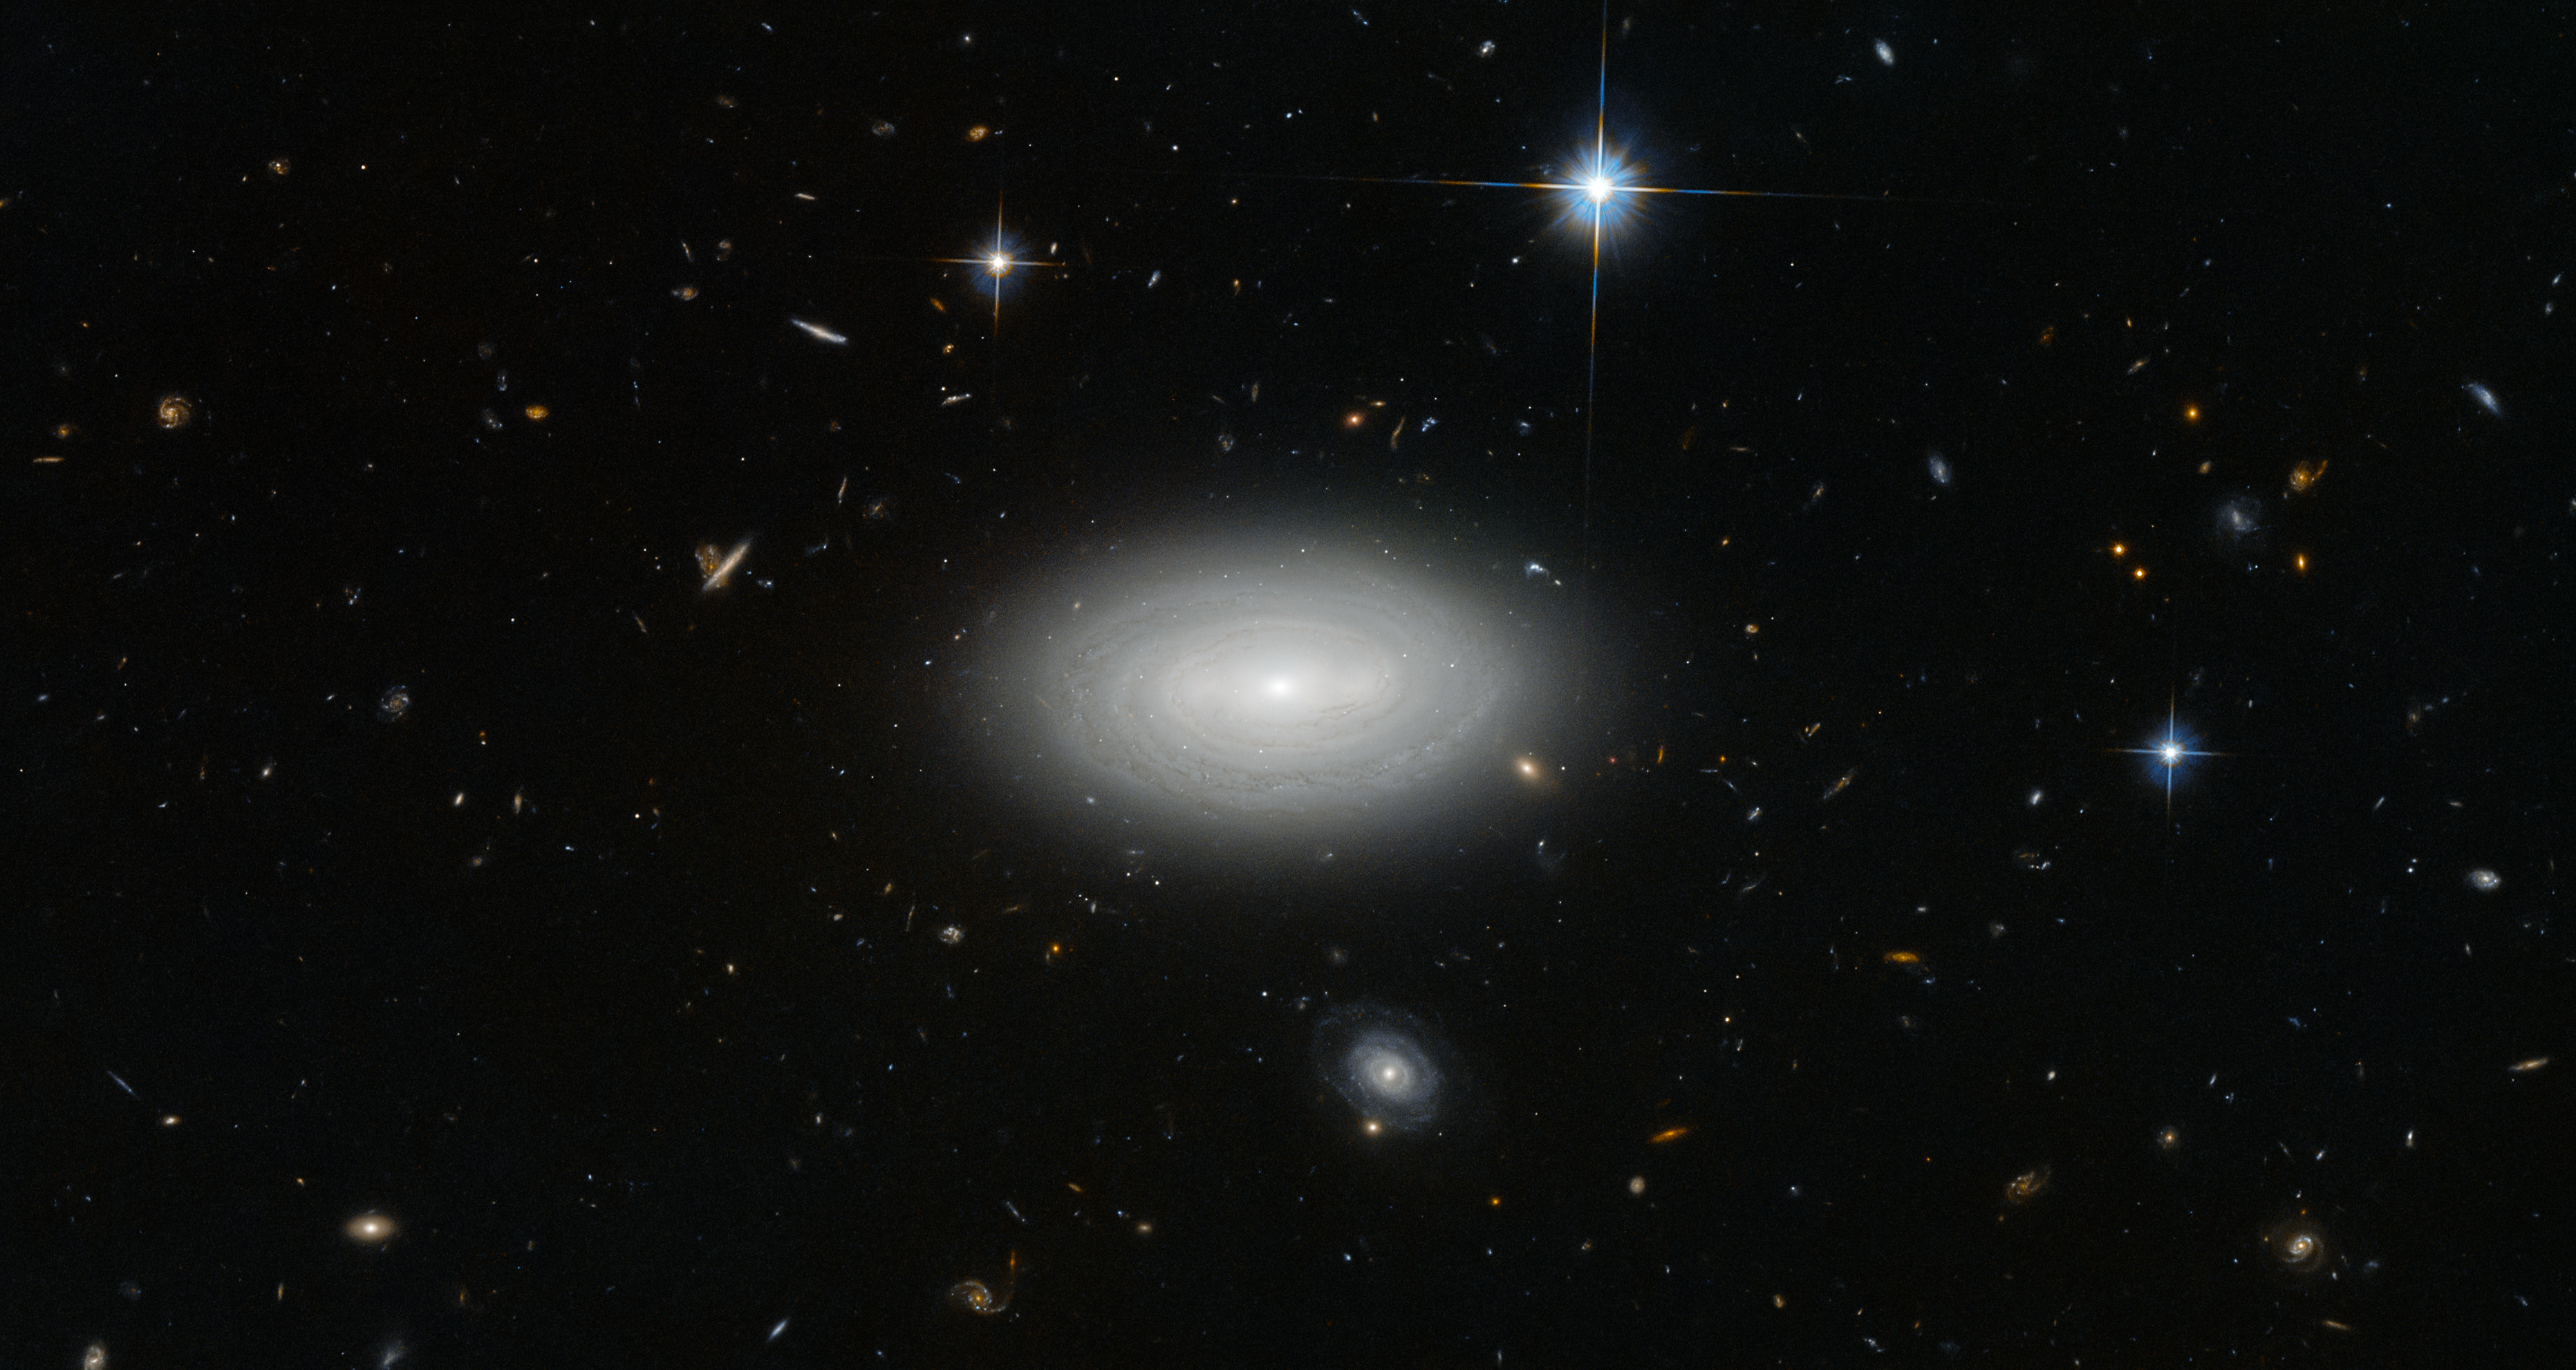
\includegraphics[width=\textwidth]{void.jpg}
        \caption{Example of \textit{undisturbed} morphology, MCG+01-02-015
    (Credit: ESA/Hubble \& NASA and N. Gorin (STScI))}
    \label{subfig: void}
\end{subfigure}%
~
\begin{subfigure}[t]{0.5\textwidth}
    \centering
    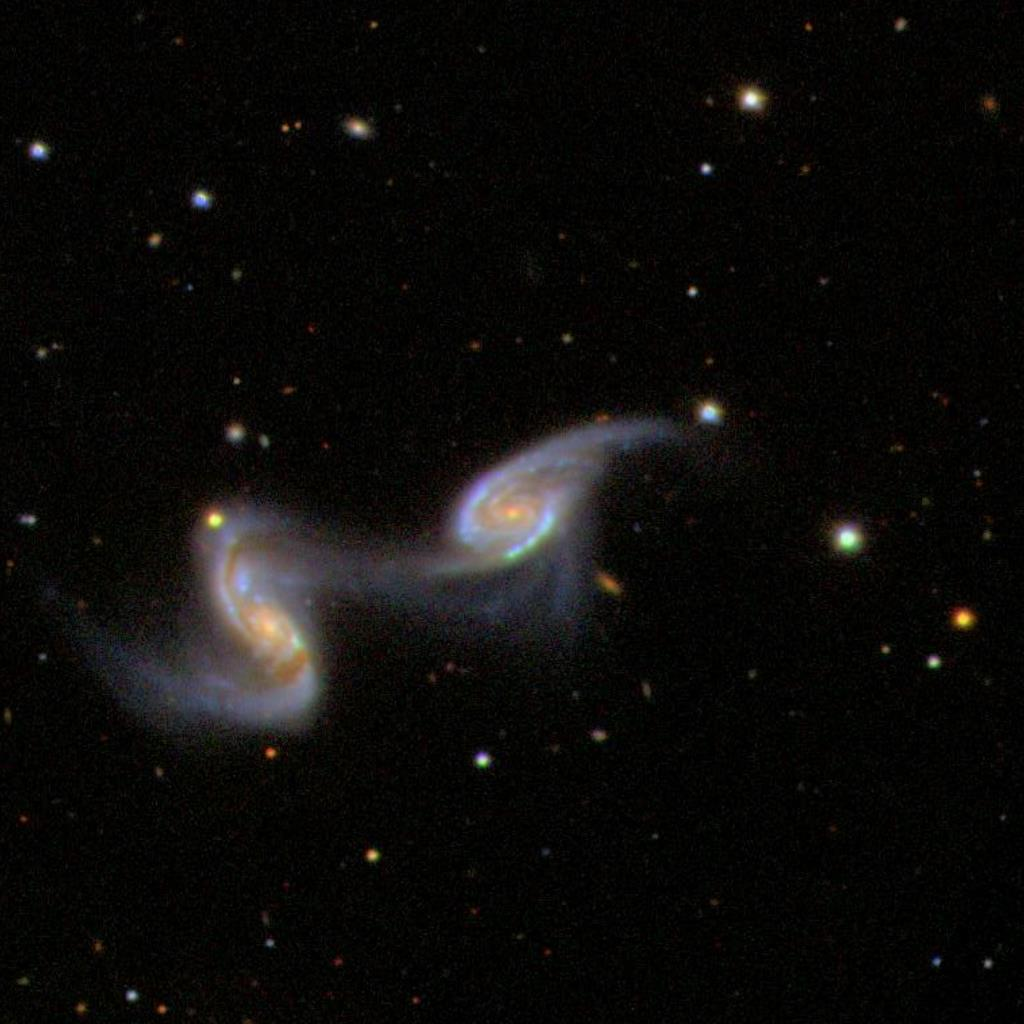
\includegraphics[width=\textwidth]{main_target.jpg}
    \caption{Example of \textit{disturbed} morphology, SDSS DR7 image of
587722984435351614. This target is part of the Galaxy Zoo: Mergers data set.}
\label{subfig: main}
    \end{subfigure}
    \caption[Comparison between undisturbed and disturbed
    morphologies]{Comparison between undisturbed and disturbed morphologies}
    \label{fig: main}
\end{figure}

Optical and spectroscopic observations can readily yield accurate measurements
of the final positions of the galaxies in a merger, and occasionally the radial
velocities of the members of a system can be observed as well. However,
the primary interest
lies in the mechanisms that result in the observed bridges and tails; this
immediately suggests the need to find precisely the final positions in space,
the overall velocity field of system, and the angular orientations of the system
with respect to our position in space. For this reason, much work has been done
in the last 70 years to advance simulations of interacting systems, and further,
to optimize the existing simulations for better convergence on solutions.


%\todo[inline]{
%  \textbf{ITEMS TO CONSIDER ADDING TO INTRODUCTION:}
%  Many of these items were discussed after the introduction had been tidied up
%  in its current form. These will be added at a later date once there has been
%  more time to read into these topics.
%  \begin{itemize}
%	\item Typically, starburst galaxies (galaxies that are in the midst of
%	  heavy star formation) are observed in the midst of a merger. Much of the
%	  work done in improving simulations of interacting galaxies is done in
%	  support of research into other mechanisms in galactic evolution; the role
%	  of mergers in changing the distribution of the star population is commonly
%	  referenced as a potential source of star formation.
%	\item Hierarchical mergers in galactic evolution (as in the evolution of
%	  galaxies from their initial generations to those we observe now.
%	  \begin{itemize}
%		\item First generation $\to$ quasars $\to$ AGNs $\to$ modern galaxies
%	  \end{itemize}
%	\item The role of mergers in cosmological evolution as a whole.
%\end{itemize}}
